\chapter{\texorpdfstring{$\bm{\lambda}$}{} Lambda calculus}

Due to Haskell's \textbf{laziness}, functions and data constructors don’t evaluate their
arguments until they need them.
In several languages there are forms of lazy evaluations (\texttt{if-then-else}, shortcutting \texttt{\&\&} and \texttt{||}).

\section{Syntax}

\lstset{
   language=Haskell,
   literate={% replace strings with symbols
{->}{{$\to$}}{2}
{lambda}{{$\lambda$}}{1}
}}

\begin{lstlisting}
   t ::= x | lambda x.t | t t' | (t)
\end{lstlisting}
\begin{itemize}
   \item \lstinline|x| variable, name, symbol,...
   \item \lstinline|lambda x.t| abstraction, defines an anonymous function
   \item \lstinline|t t'| application of function \lstinline|t| to argument \lstinline|t'|
\end{itemize}

We say that an occurrence of $x$ is \textbf{free} in a term t if it is \textbf{not} in the body of an abstraction $\lambda x. t$, otherwise it is \textbf{bound};
$\lambda x$ instead is a \textbf{binder}.\\
{Examples\ns
\begin{itemize}
   \item 
   $\lambda z. \lambda x. \lambda y. x (y z)$\\
   \item $(\lambda x. x) x$
\end{itemize}}

Terms without free variables are \textbf{combinators}.
Identity function: $id = \lambda x. x$\\
First projection: $fst = \lambda x. \lambda y. x$.

\subsection*{\texorpdfstring{\bm{$\beta $}}{}-Reduction}
$\beta $-reduction, i.e. \textit{function application}, also called \textbf{redex}:
\[(\lambda x.t)t' = t[t'/x]\]
\labelitemize{
   \color{gray} \textit{Examples}
}{
   \begin{align}
      (\lambda  x. x) y &\longrightarrow y\\
      (\lambda  x. x (\lambda  x. x) ) (u r) &\longrightarrow u r (\lambda  x.x)\\
      \label{eq:lambda_ex3}(\lambda  x. (\lambda w. x w)) (y z) &\longrightarrow \lambda w. y z w\\
      \Omega -combinator \qquad (\lambda  x. x x)(\lambda x. x x) &\longrightarrow (\lambda x. x x) (\lambda x. x x)
   \end{align}
}

Note that in the example \ref{eq:lambda_ex3}, the variable $x$ is bound in the outer $\lambda$-abstraction, is the same $x$ of the inner one. Besides, note that the parameters are substituted first in the outer $\lambda$-abstraction, then in the inner one.

\section{Functions and lambdas}
We can express most aspects of functional languages using $\lambda$-calculus.

A definition of a function with a single argument
associates a name with a $\lambda$-abstraction,
while
a function with several arguments is equivalent to a
sequence of $\lambda$-abstractions
\begin{lstlisting}
   f x = <exp> -- is equivalent to
   f = lambda x.<exp>
   
   f(x,y) = <exp> -- is equivalent to
   f = lambda x. lambda y.<exp>

   -- Curriend and uncurried functions
   curry :: ((a, b) -> c) -> a -> b -> c
   curry f x y = f(x,y)
   uncurry :: (a -> b -> c) -> (a, b) -> c
   uncurry f (x,y) = f x y
\end{lstlisting}

\section{Well-known functions}
\begin{figure}[htbp]
   \centering
   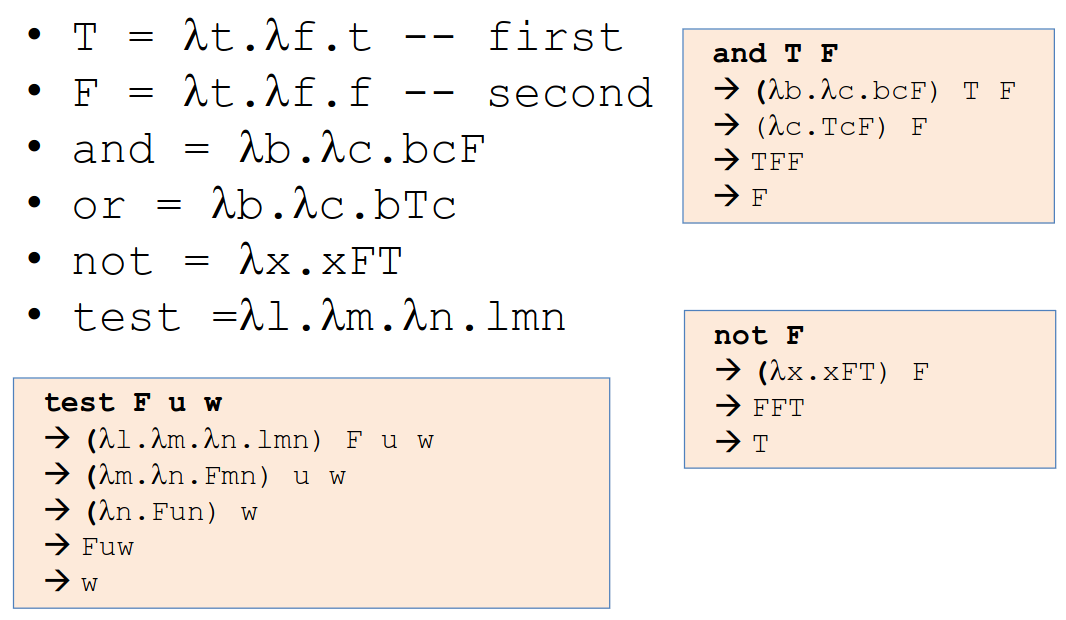
\includegraphics{images/lambda_booleans.png}
   \caption{Church Booleans using $\lambda$-calculus}
   \label{fig:lambda_booleans}
\end{figure}

\labelitemize{
   \textit{\textbf{Pair} function}
}{
   \begin{align*}
      \textit{pair} &= \lambda f.\lambda s.\lambda b.b\ f\ s\\
      \textit{fst} &= \lambda p.p\ T\\
      \textit{snd} &= \lambda p.p\ F\\
   \end{align*}
   \begin{align*}
      fst (pair u w)\\
      \longrightarrow &\quad (\lambda p.p\ T) (pair\ u\ w)\\
      \longrightarrow &\quad (pair\ u\ w)\ T\\
      \longrightarrow &\quad (\lambda f.\lambda s.\lambda b.b\ f\ s)\ u\ w T\\
      \longrightarrow &\quad (\lambda s.\lambda b.b\ u\ s)\ w\ T\\
      \longrightarrow &\quad (\lambda b.b\ u\ w)\ T\\
      \longrightarrow &\quad T\ u\ w\\
      \longrightarrow &\quad u
   \end{align*}
}
\labelitemize{
   \textit{Church \textbf{Numerals}}
}{
   \begin{align}
      0 &= \lambda s. \lambda z. z\\
      1 &= \lambda s. \lambda z. s\ z\\
      2 &= \lambda s. \lambda z. s\ (s\ z)\\
      3 &= \lambda s. \lambda z. s\ (s (s\ z))
   \end{align}
   
   \textit{Numerals} \textit{n} takes a function \textit{s} as argument
   and returns the \textit{n-th} composition
   of \textit{s} with itself, $s^n$.\\
   $succ = \lambda n. \lambda s. \lambda z. s (n s z)$ hence allows to compute the successor of 2, by substituing the -identifier- ``2'' with its numeral and viceversa.
}
\begin{align*}
   &\text{Given:} \quad& \text{succ} &= \lambda n. \lambda s. \lambda z. s (n \, s \, z) \\
   &\text{Compute:} \quad& \text{succ} \, 2 &= (\lambda n. \lambda s. \lambda z. s (n \, s \, z)) \, 2 \\
   &\text{Substitute } n \text{ with } 2: \quad& &= \lambda s. \lambda z. s (2 \, s \, z) \\
   \cline{1-4}
   &\text{Substitute } 2 \text{ with its Church numeral:} \quad& 2 &= \lambda s. \lambda z. s (s z) \\
   &\text{Evaluate } 2 \, s \, z: \quad& 2 \, s \, z &= (\lambda s. \lambda z. s (s z)) \, s \, z \\
   &&&= s (s z) \\
   \cline{1-4}
   &\text{Substitute back into the expression for succ:} \quad& &=\lambda s. \lambda z. s (s (s z))\\
   &\text{Which is the Church numeral for 3:} \quad& &= 3
   \end{align*}
\section{Fix-point \textit{Y} combinator}

The following \textit{fix-point combinator \textbf{Y}}, when applied to a function R,
returns a \textbf{fix-point} of R, i.e. $R(YR) = YR$

\begin{align}
   Y =& (\lambda y.(\lambda x.y(x\ x))(\lambda x.y(x\ x)))\\
   \begin{split}
      YR =& (\lambda x.R(x\ x))(\lambda x.R(x\ x))\\
         =& R((\lambda x.R(x\ x))(\lambda x.R(x\ x)))\\
         =& R(YR)
   \end{split}
\end{align}

\section{Evaluation ordering}
Consider the two following ways of evaluating a redex,
but remember that \textit{regardless} of the evaluation order,
the evaluation result is only one,
and it is \textbf{unique}\footnotemark
\begin{paracol}{2}
   \colfill
   \textbf{Applicative order} evaluation implies eager evaluation of arguments before applying them to the function
   \begin{lstlisting}
      (lambda x.(+ x x)) (+ 3 2)
      -> (lambda x.(+ x x)) 5
      -> (+ 5 5)
      -> 10
   \end{lstlisting}
   \colfill

   \switchcolumn
   \textbf{Normal order} evaluation implies functions to be evaluated first,
   and delay argument evaluation only when needed.
   Note that this may lead to multiple re-evaluations of the same argument.
   \begin{lstlisting}
      (lambda x.(+ x x)) (+ 3 2)
      -> (+ (+ 3 2) (+ 3 2))
      -> (+ 5 (+ 3 2))
      -> (+ 5 5)
      -> 10
   \end{lstlisting}
\end{paracol}
\footnotetext[1]{Proved by Church and Rosser}
Haskell realizes \textbf{lazy evaluation} by using \textbf{call by need} parameter passing: 
an expression passed as
argument is bound to the formal parameter, but it is
evaluated \textit{only if} its value is \textbf{needed}.
Besides, 
the argument is evaluated \textit{only} the \textbf{first time}, using
the \textbf{memoization} technique: the result is saved and
further uses of the argument do not need to re-evaluate it.

Combined with \textbf{lazy data constructors}, this allows to
construct \textit{potentially \textbf{infinite} data structures} and to call
\textit{infinitely recursive} functions without necessarily causing non-termination.
\note{
   Note: lazy evaluation works fine with purely \textbf{functional languages}.
   Side effects such as IO operations force the programmer to reason about the order in which things happen,
   which not predictable in lazy languages.
   We will address this fact when introducing Haskell's IO-\textit{Monad}.
}

\section{Value vs Reference model}
Consider the assignment $a = b$:
$a$ is an \texttt{l-value} denoting a location, while $b$ is any syntactically correct expression with a type compatible to the type of $a$.
{Depending on the model adopted by the language, two things may happen:\ns
\begin{itemize}
   \item \textbf{Value model}: $b$ value is copied into the location of $a$.
   \note{Most imperative languages use this model.}
   \item \textbf{Reference model}: a reference -to the location of- $b$ is copied onto $a$. TThis results in shared data values via multiple references.
   \note{Haskell, LISP, ML, Scheme, and Smalltalk use this model.}
   \item[-] Java uses the value model for built-in types and the reference model for class instances
   \item[-] C\# uses value model for value types, reference model for reference types
\end{itemize}}

{Note that there is a subtle difference between \textit{reference} and \textit{pointer}:\ns
\begin{itemize}
	\item A reference to \texttt{X} is the address of the (base) cell where \texttt{X} is stored
	\item A pointer to \texttt{X} is a location containing the address of \texttt{X}
\end{itemize}}
\nl

\textbf{Call by name} is a parameter passing mechanism where the actual parameter is passed as it is, and the formal parameter is substituted with the actual parameter in the function body.
This was used in Algol 60, it is powerful, but very difficult to read and debug (think of $\lambda$-calculus\dots).\\
In this mechanism arguments are passed as a closure (``thunk'') to the subroutine and re-evaluated every time they are used.

\section{Post-lecture Takeaway message}
While discussing with the professor after the lecture,
an important intuition emerged about evaluation an memoization.
\begin{lstlisting}
   a = 5
   b = a + 3
\end{lstlisting}
b would evaluate to 8 but it is not evaluated until it is strictly necessarily.

\begin{lstlisting}
   a = 5
   b = a + 3
   a = 2
   -- b?
\end{lstlisting}
Someone may think that due to lazy evaluation,
b would now evaluate to 5.
However, this is \textit{\textbf{NOT}} Haskell's case.
Due to \textbf{memoization},
even if \lstinline|b = a + 3| doesn't get evaluated,
the current value of \texttt{a} is memoized and its re-definition doens't affect b evaluation.
Thus this snippet code leads \texttt{b} to be evaluated as \texttt{8},
regardless of \texttt{a} redefinition.
\begin{lstlisting}
   a = 5
   b = a + 3
   a = 2
   b
   > 8
\end{lstlisting}
